% Reservation prices for successive units, market price, and consumer surplus.
% Compile to SVG:  latex wtp_steps.tex && dvisvgm --no-fonts wtp_steps.dvi -o ../wtp_steps.svg
\documentclass[tikz,border=6pt]{standalone}
\usepackage[scaled]{helvet}
\renewcommand{\familydefault}{\sfdefault}
\usetikzlibrary{arrows.meta}
\definecolor{blu}{HTML}{3B6EA8}
\definecolor{yel}{HTML}{F2C94C}
\definecolor{rd}{HTML}{C62828}
\definecolor{accent}{HTML}{2E7D32}
\begin{document}
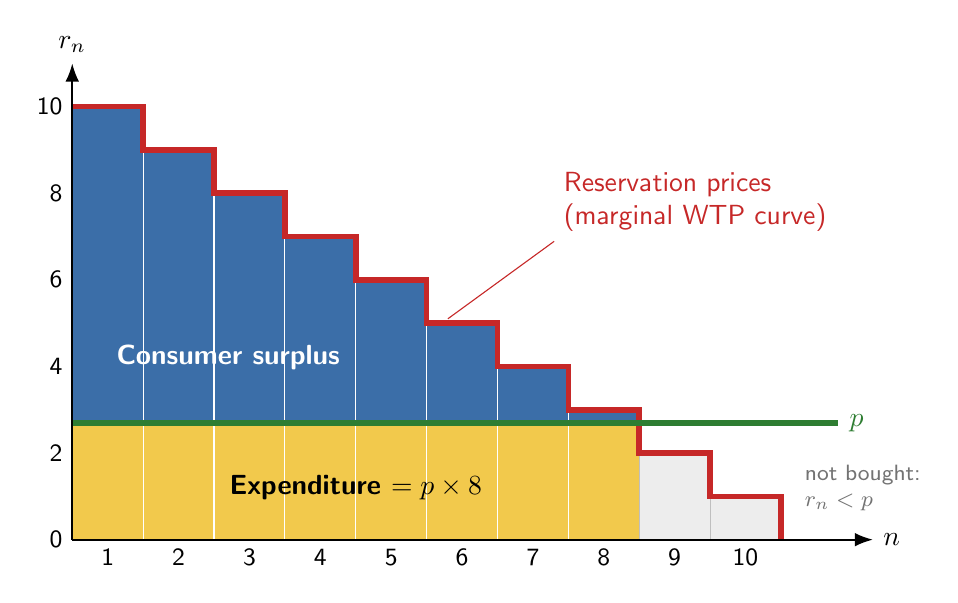
\begin{tikzpicture}[x=0.9cm, y=0.55cm]
  \def\p{2.7}
  % bars: unit n has reservation price r_n = 11 - n
  \foreach \n in {1,...,10} {
    \pgfmathsetmacro{\r}{11-\n}
    \ifnum\n<9
      \fill[yel, draw=white] (\n-1,0) rectangle (\n,\p);
      \fill[blu, draw=white] (\n-1,\p) rectangle (\n,\r);
    \else
      \fill[black!7, draw=black!25] (\n-1,0) rectangle (\n,\r);
    \fi
    \node[below, font=\small] at (\n-0.5,0) {\n};
  }
  % step curve
  \draw[rd, line width=2pt]
    (0,10) \foreach \n in {1,...,10} { -- (\n,11-\n) -- (\n,10-\n) };
  % price
  \draw[accent, line width=2pt] (0,\p) -- (10.8,\p) node[right] {$p$};
  % axes
  \draw[-{Latex}, thick] (0,0) -- (11.3,0) node[right] {$n$};
  \draw[-{Latex}, thick] (0,0) -- (0,11) node[above] {$r_n$};
  \foreach \y in {0,2,...,10} \node[left, font=\small] at (0,\y) {\y};
  % labels
  \node[white, font=\bfseries] at (2.2,4.2) {Consumer surplus};
  \node[font=\bfseries] at (4,1.2) {Expenditure $= p \times 8$};
  \node[rd, align=left, anchor=west] (lab) at (6.8,7.8) {Reservation prices\\(marginal WTP curve)};
  \draw[rd] (lab.south west) -- (5.3,5.1);
  \node[black!55, font=\footnotesize, align=left, anchor=west] at (10.2,1.2) {not bought:\\$r_n < p$};
\end{tikzpicture}
\end{document}
